\begin{questions}
\question{
  Si chiede di progettare un sistema automatico per l'attracco di 4 navi di tipologia diversa in due differenti punti di sbarco di un porto, le quali sono individuate tramite le seguenti lettere J, C, P e S.

  Tutte quante possono arrivare contemporaneamente al porto, ma ognuna ha una diversa priorità rispetto alle altre:
    \begin{itemize}
        \item J ha una priorità maggiore di tutte le altri navi;
        \item C ha una priorità maggiore solo di P e S;
        \item P ha priorità maggiore di S.
    \end{itemize}
  Quest'ultima può essere riassunta tramite la seguente formula $J > C > P > S$. \\
  Il sistema di attracco è gestito tramite 4 differenti variabili X, Y, Z e W secondo la codifica riportata in Tabella \ref{tab:codifica}.

    \begin{table}[h!]
        \centering
            \begin{tabular}{ |p{1cm}||p{1cm}|p{1cm}|p{1cm}| p{3cm}|  }
                 \hline
                 \multicolumn{5}{|c|}{Codifica attracco navi} \\
                 \hline
                 X & Y & Z  & W& Navi\\
                 \hline
                0   & 0  &0&  0& Nessun attracco\\
                 0&   0  & 0   &1 & J\\
                 0 &0 & 1&  0 &C\\
                 0 & 1 & 0 & 0 & P\\
                 1 & 0 & 0 & 0 & S\\
                 0 & 0 & 1 & 1 &JC\\
                 0 & 1 & 0 &  1 &JP\\
                 1 & 0 & 0 &  1 &JS\\
                 0 & 1 & 1 & 0 &CP\\
                 1 & 0 & 1 &  0 &CS\\
                 1 & 1 & 0 &  0 &PS\\ 
                 \hline
            \end{tabular}

        \label{tab:codifica}
    \end{table}

}

\newpage
    \begin{solution}
       \mysection{Formulazione}
        Creazione della tabella di verità.
        
            \begin{center}
              \begin{tabular}{cccc|cccc|c}
                J & C & P & S & X & Y & Z & W & Attracco\\
                \hline
                0 & 0 & 0 &0 & 0 & 0 & 0 &0 & Nessuna\\
                0 & 0 & 0 &1 & 1 & 0 & 0 &0 & S\\
                0 & 0 & 1 & 0 & 0 & 1 & 0 & 0 & P\\
                0 & 0 & 1 & 1 & 1 & 1 & 0 & 0 & PS \\
                0 & 1 & 0 & 0 & 0 & 0 & 1 & 0 & C \\ 
                0 & 1 & 0 & 1 & 1 & 0 & 1 & 0 & CS \\
                0 & 1 & 1 & 0 & 0 & 1 & 1 & 0 & CP \\
                0 & 1 & 1 & 1 & 0 & 1 & 1 & 0 & CP \\
                1 & 0 & 0 & 0 & 0 & 0 & 0 & 1 & J \\
                1 & 0 & 0 & 1 & 1 & 0 & 0 & 1 & JS \\
                1 & 0 & 1 & 0 & 0 & 1 & 0 & 1 & JP \\
                1 & 0 & 1 & 1 & 0 & 1 & 0 & 1 & JP \\
                1 & 1 & 0 & 0 & 0 & 0 & 1 & 1 & JC \\
                1 & 1 & 0 & 1 & 0 & 0 & 1 & 1 & JC \\
                1 & 1 & 1 & 0 & 0 & 0 & 1 & 1 & JC \\
                1 & 1 & 1 & 1 & 0 & 0 & 1 & 1 & JC\\
              \end{tabular}
            \end{center}
            
        \mysection{Ottimizzazione}
            Creazione delle Mappe di Karnaugh.
            \begin{enumerate}
                    \item Mappa di Karnaugh per X.
                    
                        \begin{center}
                            \begin{karnaugh-map}[4][4][1][$JC$][$PS$]
                                \manualterms{0,0,0,0,1,1,1,0,0,0,0,0,1,0,0,0}
                                \implicant{4}{12}
                                \implicant{4}{5}
                                \implicantedge{4}{4}{6}{6}
                             \end{karnaugh-map}
                        \end{center}
                        \[ X = S \overline{CP}  +  S \overline{JP} + S \overline{JC}  \]
                        
                    \item Mappa di Karnaugh per Y.
                    
                        \begin{center}
                            \begin{karnaugh-map}[4][4][1][$JC$][$PS$]
                                \manualterms{0,0,0,0,0,0,0,0,1,1,1,0,1,1,1,0}
                                \implicant{12}{9}
                                \implicantedge{12}{8}{14}{10}
                             \end{karnaugh-map}
                        \end{center}
                    \[ Y = P \overline{J}  +  P \overline{C} \]
                    
                     \item Mappa di Karnaugh per Z.
                    
                        \begin{center}
                            \begin{karnaugh-map}[4][4][1][$JC$][$PS$]
                                \manualterms{0,1,0,1,0,1,0,1,0,1,0,1,0,1,0,1}
                                \implicant{1}{11}
                             \end{karnaugh-map}
                        \end{center}
                    \[ Z = C \]
                    
                    
                    \item Mappa di Karnaugh per W.
                    
                        \begin{center}
                            \begin{karnaugh-map}[4][4][1][$JC$][$PS$]
                                \manualterms{0,0,1,1,0,0,1,1,0,0,1,1,0,0,1,1}
                                \implicant{3}{10}
                             \end{karnaugh-map}
                        \end{center}
                    \[ W = J \]
            \end{enumerate}
            
            \mysection{Disegno del circuito}
            Disegno del circuito combinatorio non minimizzato.
             %%%%%%%%%%%%  DA FARE %%%%%%%%%%%%%
                    \begin{center}
                        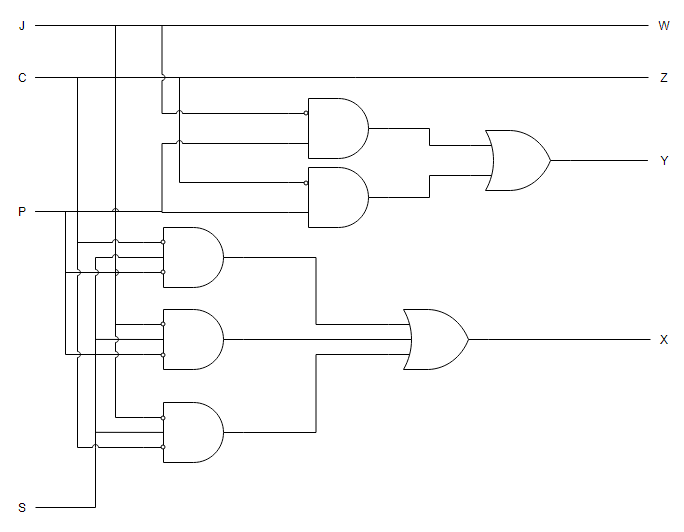
\includegraphics[width=13cm, keepaspectratio]{img/carpi_diagramma_no_min.png}
                    \end{center}
            \newpage
            Disegno del circuito combinatorio minimizzato tramite le seguenti formule:    
                \[ X = S(\overline{CP} + \overline{JP} + \overline{JC})\]
                \[ Y = P(\overline{J} +\overline{C})\]
                \[ Z = C \]
                \[ W = J \]
                    \begin{center}
                            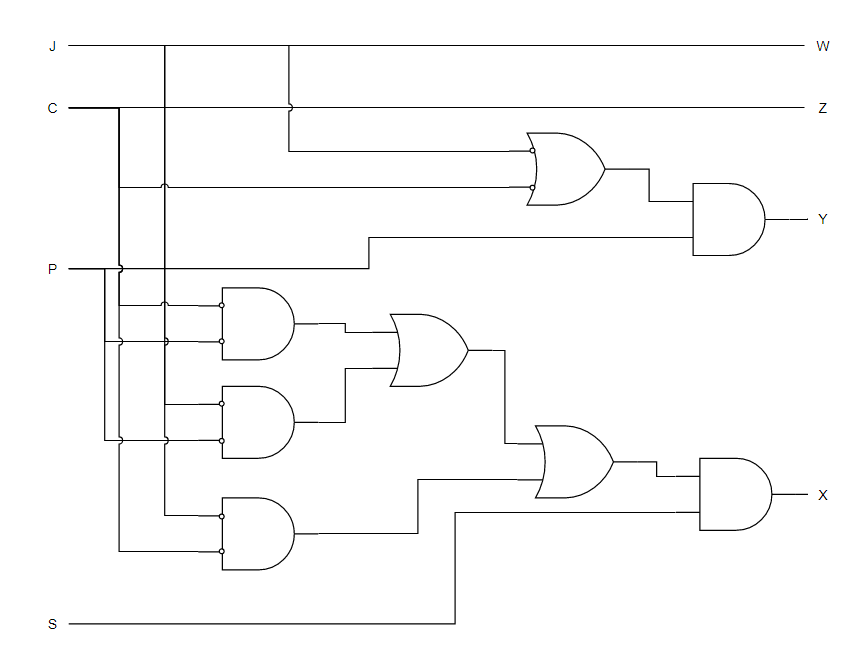
\includegraphics[width=13cm, keepaspectratio]{img/carpi_diagramma.png}
                    \end{center}
                 

    \end{solution}
\end{questions}